% !TeX root = ../Thesis.tex

\chapter{Introduction}

\begin{figure}[tbp]
\centering
\begin{tikzpicture}
% Light
\fill[red, path fading=fade left] (-3,-0.75/2.0) rectangle (3,0.75/2.0); % Gain
\fill[red, fill opacity=0.25] (-4,-0.75/2.0) rectangle (-3,0.75/2.0); % Left
\fill[red] (3,-0.75/2.0) rectangle (4,0.75/2.0); % Right
\fill[red] (4,-0.2) rectangle (6,0.2); % Right

\draw[fill=Goldenrod] (-4,1) rectangle (-3.8,-1); % Left
\fill[pattern=north west lines, pattern color=Goldenrod] (3.8,-0.2) rectangle (4,0.2); % Right Mid
\draw[fill=Goldenrod] (3.8,0.2) rectangle (4,1); % Right Top
\draw[fill=Goldenrod] (3.8,-0.2) rectangle (4,-1); % Right Bottom
\draw[pattern=mydots, pattern color=Purple] (-3,-0.75) rectangle (3,0.75); % Gain
\draw (-4,1) -- (4,1); % Top
\draw (-4,-1) -- (4,-1); % Bottom

% Labels
\draw[->, >=stealth, thick] (3.5,-1.5) -- (3.9,-0.75) node[pos=-0.3] {Partially Reflecting Mirror};
\draw[->, >=stealth, thick] (-3.5,-1.5) -- (-3.9,-0.75) node[pos=-0.3] {Mirror};
\draw[->, >=stealth, thick] (-1,-1.43) -- (-1,-0.5) node[pos=-0.3] {Gain Medium};
\draw[->, >=stealth, thick] (5,1.2) -- (5.5,0) node[pos=-0.3] {Laser Output};
\draw[->, >=stealth, thick] (0,1.2) -- (-3.5,0);
\draw[->, >=stealth, thick] (0,1.2) -- (3.5,0);
\draw (0,1.5) node {Laser Light};
\end{tikzpicture}
\caption{Depiction of a standard laser. A majority of the light is continually reflected by the two mirrors with a small portion escaping to become the output. The light is amplified by the gain medium with each pass.}
\label{fig:laser}
\end{figure}

The word laser was originally an acronym for \emph{Light Amplification by Stimulated Emission of Radiation}. The cavity of a standard laser---such as a HeNe laser---is composed of four main components: a highly reflective mirror, a partially reflecting mirror, something to supply the energy, and the amplifying, or gain, medium. The two mirrors are at opposite ends of the cavity and serve to contain most of the light in the cavity while allowing a small amount to exit---this is the output of the laser, this is shown in Figure \ref{fig:laser}. The energy is generally supplied by either an external light source, or an electric field. The amplifying medium for a single frequency laser typically consists of gases, such as Helium and Neon, or a crystal, such as \gls{ndyag}. \\

\begin{figure}[tbp]
\centering
% !TeX root = ../Thesis.tex

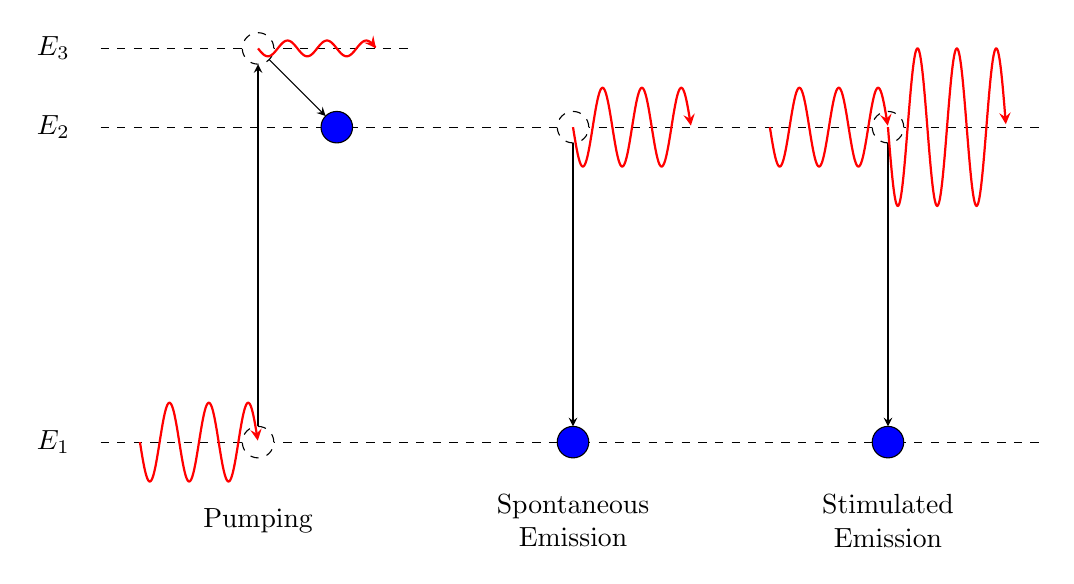
\begin{tikzpicture}
% Energy levels
\draw [dashed] (0,0) -- (12,0) node [pos = -0.05] {$E_1$};
\draw [dashed] (0,4) -- (12,4) node [pos = -0.05] {$E_2$};
\draw [dashed] (0,5) -- (4,5) node [pos = -0.15] {$E_3$};

% Transition arrows
\draw[->, >=stealth] (2,0.2) -- (2,4.8);
\draw[->, >=stealth] (2,5) -- (3-0.2*0.707,4+0.2*0.707);
\draw[<-, >=stealth] (6,0.2) -- (6,4);
\draw[<-, >=stealth] (10,0.2) -- (10,4);

% Circles
% Bottom
\filldraw[fill=white, draw=black, dashed] (2,0) circle (0.2);
\filldraw[fill=blue, draw=black] (6,0) circle (0.2);
\filldraw[fill=blue, draw=black] (10,0) circle (0.2);
% Top
\filldraw[fill=white, draw=black, dashed] (2,5) circle (0.2);
\filldraw[fill=blue, draw=black] (3,4) circle (0.2);
\filldraw[fill=white, draw=black, dashed] (6,4) circle (0.2);
\filldraw[fill=white, draw=black, dashed] (10,4) circle (0.2);

% Photons
\draw [domain=0.5:2, samples=250, red, thick, ->, >=stealth] plot (\x, {-0.5*sin(4*pi*deg(\x-2))});
\draw [domain=2:3.5, samples=250, red, thick, ->, >=stealth] plot (\x, {5-0.1*sin(4*pi*deg(\x-2))});
\draw [domain=6:7.5, samples=250, red, thick, ->, >=stealth] plot (\x, {4-0.5*sin(4*pi*deg(\x-6))});
\draw [domain=8.5:10, samples=250, red, thick, ->, >=stealth] plot (\x, {4-0.5*sin(4*pi*deg(\x-10))});
\draw [domain=10:11.5, samples=250, red, thick, ->, >=stealth] plot (\x, {4-sin(4*pi*deg(\x-10))});

% Labels
\node at (2, -1){Pumping};
\node [align=center] at (6, -1){Spontaneous \\ Emission};
\node [align=center] at (10, -1){Stimulated \\ Emission};
\end{tikzpicture}
\caption[Comparison of pumping, spontaneous emission, and stimulated emission.]{In pumping, incident photons are absorbed by electrons which are then excited into a much higher energy state (the electrons may also be excited by an electric field). The electrons quickly emit a low energy photon and transition down to an energy state that is still much more energetic than the original. In spontaneous emission, an electron in an excited state emits a photon and returns to the lower energy state. Finally, in stimulated emission, an incident photon interacts with an electron in an excited state, the electron donates its energy to the photon and returns to the lower energy state.}
\label{fig:emission}
\end{figure}

The atoms in the gain medium are pumped with energy raising the electrons to an excited state. For stimulated emission an incident photon triggers the emission of a photon which causes the electron to transition back to the ground state \cite{alazzawi}. This new photon is emitted with the combined energy of the previous photon as well as the electron's energy, thus, amplifying the light. Furthermore, the photon is released with the same direction and phase as the incident one, maintaining coherence \cite{alazzawi}. These processes are highlighted in Figure \ref{fig:emission}. The light perpetually bounces between the two mirrors becoming more amplified with each interaction with an excited electron and a fraction of this light is able to pass through the partially reflecting mirror to become the output of the laser. \\

Laser light has two fundamental characteristics that regular light does not. The first is that the light is highly monochromatic---the light contains (ideally) a single frequency. This is in contrast with an incandescent light bulb, for example, which emits light at all wavelengths with relative intensities given by Planck's law of black-body radiation. The other key feature is coherence, in which all the peaks and troughs of the light overlap giving very strong constructive interference---this is why laser light can be so intense. A system such as a \gls{led} does not produce laser light because, while monochromatic, the light is not coherent. The monochromatic nature is a result of how the light is generated; the frequency of the light emitted directly corresponds to the energy difference between the excited and ground states of the gain medium (as with \gls{led}s). Note that this means the operating frequency of the laser is fixed, and cannot be changed. Coherence is achieved in the laser cavity---the cavity is carefully designed so the light resonates with the length of the cavity. This causes all the peaks and troughs to align, and interfere constructively. \\

Another class of lasers are optical fibre lasers. Optical fibre lasers operate by the same principles, however, instead of the light being perpetually reflected back and forth, the light travels in a circular fashion along an optical fibre---this is a so called ring laser. Additionally, instead of the gain medium consisting of a gas or crystal, it is a length of fibre doped with a rare-earth metal. \\

\section{Tuneable Lasers}
\begin{figure}[tbp]
\centering
% !TeX root = ./Tuneable_Lasers.tex

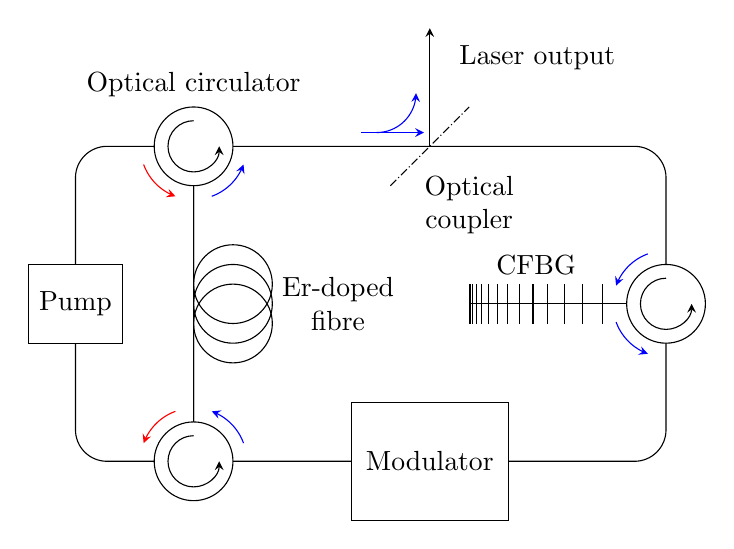
\begin{tikzpicture}
% Two laser loops
\draw [rounded corners=4mm] (0,0) rectangle ++(6,4);
\draw [rounded corners=4mm] (0,0) rectangle ++(-1.5,4);

% Gain
\draw (0.5,2.25) circle (0.5cm);
\draw (0.5,2) circle (0.5cm) node [anchor=west,xshift=0.5cm,align=center] {Er-doped \\ fibre};
\draw (0.5,1.75) circle (0.5cm);

% Modulator and pump
\filldraw[fill=white, draw=black] (2,-0.75) rectangle ++(2,1.5) node [midway] {Modulator};
\filldraw[fill=white, draw=black] (-2.1,1.5) rectangle ++(1.2,1) node [midway] {Pump};

% Coupler and output
\draw[-stealth] (3,4) -- (3,5.5) node [pos=0.75,anchor=west,xshift=0.25cm] {Laser output};
\draw[densely dashdotted] (2.5,3.5) -- (3.5,4.5) node [pos=1,anchor=north,yshift=-0.75cm,align=center] {Optical \\ coupler};

% Circulators
\filldraw[fill=white, draw=black] (6,2) circle (0.5cm);
\draw[->,>=stealth] (6,2.325) arc (90:360:0.325cm);

\filldraw[fill=white, draw=black] (0,0) circle (0.5cm);
\draw[->,>=stealth] (0,0.325) arc (90:360:0.325cm);

\filldraw[fill=white, draw=black] (0,4) circle (0.5cm) node [anchor=south,align=center,yshift=0.5cm] {Optical circulator};
\draw[->,>=stealth] (0,4.325) arc (90:360:0.325cm);

% Arrows
\draw [->,>=stealth,domain=20:70,blue] plot ({0.675*cos(\x)}, {0.675*sin(\x)});
\draw [->,>=stealth,domain=110:160,red] plot ({0.675*cos(\x)}, {0.675*sin(\x)});
\draw [->,>=stealth,domain=110:160,blue] plot ({6+0.675*cos(\x)}, {2+0.675*sin(\x)});
\draw [->,>=stealth,domain=200:250,blue] plot ({6+0.675*cos(\x)}, {2+0.675*sin(\x)});
\draw [->,>=stealth,domain=200:250,red] plot ({0.675*cos(\x)}, {4+0.675*sin(\x)});
\draw [->,>=stealth,domain=290:340,blue] plot ({0.675*cos(\x)}, {4+0.675*sin(\x)});

\draw [->,>=stealth,domain=270:360,blue] plot ({2.325+0.5*cos(\x)}, {4.675+0.5*sin(\x)});
\draw [->,>=stealth,blue] (2.125, 4.675-0.5) -- (2.325+0.6, 4.675-0.5);

% Grating
\draw (5.5,2) -- (3.5,2) node [pos=0.5,anchor=south,yshift=0.25cm,xshift=-0.15cm] {CFBG};
\foreach \i in {0,...,13}
	\draw (3.5 + \i*\i/100,1.75) -- (3.5 + \i*\i/100,2.25);

\end{tikzpicture}
\caption[Typical cavity of a tuneable laser.]{Typical cavity of a fibre based tuneable laser. The pulses travel clockwise around each loop.}
\label{fig:cavity}
\end{figure}

A tuneable laser has the ability to vary its wavelength, and hence frequency, by up to about 100 nanometres \cite{bohun, burgoyne2010, yamashita}. Tuneable lasers can lase at all of these different frequencies simultaneously. This tuneability is quite useful and has applications in spectroscopy and high resolution imaging such as coherent anti-Stokes Raman spectroscopy and optical coherence tomography \cite{bohun, burgoyne2014, yamashita}, as well as communications and diagnostics of ultra fast processes \cite{silfvast}. A typical tuneable laser cavity is shown in Figure \ref{fig:cavity}. The gain medium is still excited by an external power source, and the output passes through a partially reflecting mirror. However, a tuneable laser also contains a few additional components, each of which will be described in the following subsections. 

\subsection{Optical Coupler and Laser Output}
The optical coupler is a device that splits its input into two outputs---one continues through the laser cavity, while the other exits the cavity to become the output of the laser. There are multiple devices that can accomplish this, however, the simplest is a partially reflecting mirror \cite{alazzawi}. These mirrors are characterized by their reflection coefficient, $R$. In the schematic shown in Figure \ref{fig:cavity}, the part of the signal that is reflected exits the cavity, whereas the part of the signal transmitted remains within the cavity. \\

\subsection{\glslink{fbg}{Fibre Bragg Grating}}
\label{sec:fbg}
A \gls{fbg} is an optical fibre where the refractive index varies periodically along its length \cite{ferreira}. To achieve this periodicity, typically silica fibres are doped with Germanium which when exposed to intense \gls{uv} light permanently alters the refractive index of the core \cite{becker, starodoumov}. The photosensitivity of the optical fibres can be increased by more than an order of magnitude by the Germanium doping \cite{becker, ferreira}. \\

\begin{figure}[p]
\centering
\begin{subfigure}{\textwidth}
\centering
% !TeX root = ../Thesis.tex

\begin{tikzpicture}
\draw[pattern=north east lines, pattern color=blue] (-4,0.5) rectangle (4,1); % Top Insulation
\draw[pattern=north west lines, pattern color=blue] (-4,-0.5) rectangle (4,-1); % Bottom Insulation
\draw[pattern=mydots, pattern color=OliveGreen] (-4,-0.5) rectangle (4,0.5); % Core
\draw[fill=black] (-2,1.5) rectangle (2,1.75); % Phase Mask top

\foreach \i in {0,...,7}
  \draw[magenta, thick] (-1.75 + \i/2,5) -- (-1.75 + \i/2,1.5);

\foreach \i in {0,...,3}{
  % Phase mask teeth
  \draw[fill=black] (-2 + \i,1.25) rectangle (-1.75 + \i,1.5); 
  \draw[fill=black] (-1.25 + \i,1.25) rectangle (-1 + \i,1.5);
  % Rays
  \draw[->, >=stealth, magenta, thick] (-1.75 + \i,1.5) -- (-1.25 + \i,-1.5);
  \draw[->, >=stealth, magenta, thick] (-1.25 + \i,1.5) -- (-1.75 + \i,-1.5);
}
% Labels
\draw[->, >=stealth, thick] (3,-1.5) -- (2,0) node[pos=-0.2] {Ge-Doped Core};
\draw[->, >=stealth, thick] (-3,-1.5) -- (-2,-0.75) node[pos=-0.3] {Cladding};
\draw[->, >=stealth, thick] (-3,2.5) -- (-1.75,2) node[pos=-0.4] {UV Light};
\draw[->, >=stealth, thick] (3,2.5) -- (2,1.5) node[pos=-0.2] {Phase-Mask};
\end{tikzpicture}
\caption{\textbf{Phase-Mask:} The phase-mask refracts the \gls{uv} light onto the core.}
\label{fig:phasemask}
\vspace{10mm}
\end{subfigure}
\begin{subfigure}{\textwidth}
\centering
% !TeX root = ../Thesis.tex

\begin{tikzpicture}

\draw[pattern=north east lines, pattern color=blue] (-4,0.5) rectangle (4,1); % Top Insulation
\draw[pattern=north west lines, pattern color=blue] (-4,-0.5) rectangle (4,-1); % Bottom Insulation
\draw[pattern=mydots, pattern color=OliveGreen] (-4,-0.5) rectangle (4,0.5); % Core

\foreach \i in {0,...,3}{
  % Rays
  \draw[->, >=stealth, magenta, thick] (-2.25 + \i,4.5) -- (-1.25 + \i,-1.5);
  \draw[->, >=stealth, magenta, thick] (-0.75 + \i,4.5) -- (-1.75 + \i,-1.5);
}
% Labels
\draw[->, >=stealth, thick] (3,-1.5) -- (2,0) node[pos=-0.2] {Ge Doped Core};
\draw[->, >=stealth, thick] (-3,-1.5) -- (-2,-0.75) node[pos=-0.3] {Cladding};
\draw[->, >=stealth, thick] (-3,2.5) -- (-1.82,2) node[pos=-0.4] {UV Light};
\end{tikzpicture}
\caption{\textbf{Holographic Side Exposure:} Two incident beams intersect at the core.}
\label{fig:holographic}
\end{subfigure}
\caption[Manufacture methods of fibre Bragg gratings.]{Depictions of the two most common methods for manufacturing \gls{fbg}s. The \gls{uv} light is focused on the core causing periodic constructive and destructive interference. The \gls{uv} light alters the refractive index of the core, causing a sinusoidal variation along the length.}
\label{fig:fbgmake}
\end{figure}

\gls{fbg}s can be manufactured using one of two methods---the phase-mask method \cite{agrawal2002, alazzawi, becker, starodoumov}, or the holographic side exposure method \cite{agrawal2002, alazzawi, becker, ferreira, starodoumov}---these are shown in Figure \ref{fig:fbgmake}. Both methods cause the periodic nature of the refractive index through interference. In the phase-mask method (Figure \ref{fig:phasemask}), a single beam of \gls{uv} light passes through the phase-mask which acts as a series of lenses, focusing the light onto the core---this causes a sinusoidal interference pattern. Similarly, in the holographic side exposure method (Figure \ref{fig:holographic}), two beams of \gls{uv} light are instead used to create the interference pattern. \\

The purpose of \gls{fbg}s is that they act as reflective filters \cite{agrawal2002, alazzawi, ferreira, starodoumov}. Due to the periodicity of the refractive index, light with the corresponding wavelength will be reflected with all others passing through. This wavelength is defined by the Bragg condition \cite{agrawal2002, alazzawi, becker, ferreira, silfvast, starodoumov}:
\begin{align}
\label{eq:bragg}
\lambda_B = 2 \Lambda \bar{n},
\end{align}
where $\lambda_B$ is the Bragg wavelength, $\Lambda$ is the period of the grating, and $\bar{n}$ is the average index of refraction. Ideally, only light with a wavelength of $\lambda_B$ would be reflected, however, there is a very narrow neighbourhood around $\lambda_B$ in which wavelengths are partially reflected too; the characteristic width of this region is known as the stop-band. \\

\subsubsection{\glslink{cfbg}{Chirped Fibre Bragg Grating}}
\begin{figure}[tbp]
\begin{subfigure}{0.5\textwidth}
\input{./Figures/Unchirped}
\caption{Unchirped Gaussian pulse. $\omega(x) = 3 \pi x$.}
\label{fig:unchirped}
\end{subfigure}
\begin{subfigure}{0.5\textwidth}
\input{./Figures/Chirped}
\caption{Linearly chirped Gaussian pulse. $\omega(x) = 2 (x - \pi)^2$.}
\label{fig:chirped}
\end{subfigure}
\caption[Comparison of a chirped and unchirped Gaussian pulse.]{In an unchirped pulse the frequency is constant, however, in a chirped pulse the frequency varies along the envelope. The waveforms are given by $\exp \left( -x^2/2 \right) \sin \omega (x)$.}
\label{fig:chirp}
\end{figure}

Chirp is simply the term for a signal that has a non-constant frequency across it. Figure \ref{fig:chirp} shows examples of chirped and unchirped Gaussian pulses---the most common type of chirp is linear chirp, where the frequency varies linearly across the pulse. In this case, for a spatially varying frequency, the oscillations are characterized by $\exp \left( i k(x) x \right) = \exp \left( i C x^2 \right)$, where $k(x) = Cx$ is the linear variation of the wave number, and $C$ is the chirp parameter. By using a chirped phase-mask, a \gls{cfbg} can be created. The spacial variation of the refractive index effectively creates a spacial dependence on the Bragg condition, \eqref{eq:bragg}. This causes most wavelengths to be reflected by a \gls{cfbg}, but with each wavelength satisfying the Bragg condition at a different spacial location\footnote{Note that a monotonic chirping ensures that the spacial dependence of the Bragg condition is continuous with respect to the wavelength.}. A consequence of this is that a time delay is created between wavelengths---this is depicted in Figure \ref{fig:cfbg} with the upper portion showing  the refractive index as a function of the depth. In this orientation, the red (dashed) wave is unable to penetrate as far as the blue (solid) wave since each wave is reflected where it matches the frequency of the refractive index. Each \gls{cfbg} has a bandwidth within which all frequencies are reflected at some point along the depth, alternatively, frequencies outside the bandwidth would be transmitted and lost. \\

\begin{figure}[tbp]
\centering
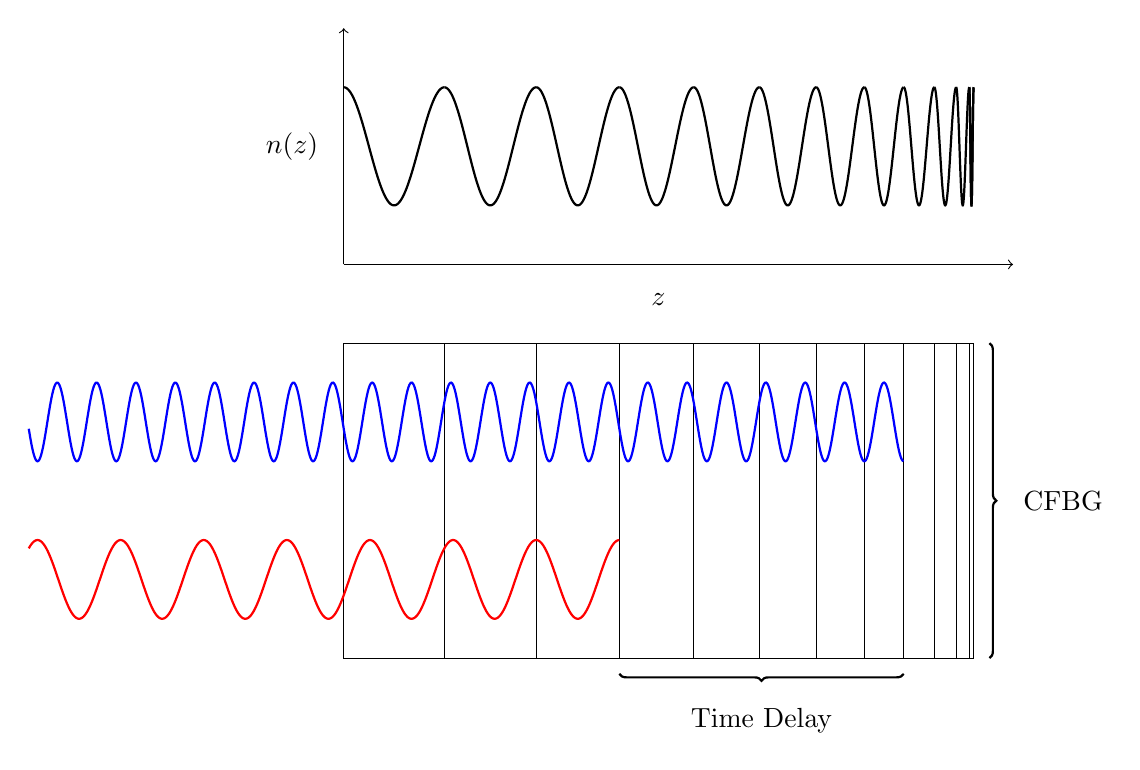
\begin{tikzpicture}
\draw (4,0) -- (12,0) -- (12,4) -- (4,4) -- cycle;
\foreach \i in {1,...,12}
  \draw (12 - 1/18*\i*\i,0) -- (12 - 1/18*\i*\i,4);
%\foreach \i in {0,...,12}
%  \draw [dashed] (12 - 1/18*\i*\i,4) -- (12 - 1/18*\i*\i,8);
\draw [domain=0:(12-16/18), samples=1000, blue, thick] plot (\x, {-0.5*cos(4*pi*(\x-(12-25/18)) r) + 3});
\draw [domain=0:(12-81/18), samples=500, red, thick] plot (\x, {0.5*cos(2*pi*36/38*(\x-(12-100/18)) r) + 1});

\draw [thick, decoration={brace, mirror, raise=0.2cm}, decorate] (7.5,0) -- (100/9,0)
node [pos=0.5,anchor=north,yshift=-0.5cm] {Time Delay};
\draw [thick, decoration={brace, mirror, raise=0.2cm}, decorate] (12,0) -- (12,4)
node [pos=0.5,anchor=west,xshift=0.5cm] {CFBG};

\draw [->] (4,5) -- (12.5,5)
node [pos=0.47,anchor=north,yshift=-0.25cm] {$z$};
\draw [->] (4,5) -- (4,8)
node [pos=0.5,anchor=east,xshift=-0.2cm] {$n(z)$};
\foreach \i in {0,...,12}
  \draw [domain=(12-\i*\i/18):(12-(\i-1)*(\i-1)/18), samples=100, black, thick] plot (\x, {3/4*cos(2*pi*36/(4*\i-2)*(\x-(12-\i*\i/18)) r) + 6.5});
\end{tikzpicture}
\caption[Chirped fibre Bragg grating.]{\Acrlong{cfbg}. The upper portion shows how the index of refraction varies along the depth. Light is reflected when the wavelength coincides with the Bragg wavelength. This causes light with different wavelengths to penetrate to different depths. In turn, dispersion is either heightened or compensated---depending on the orientation.}
\label{fig:cfbg}
\end{figure}

Furthermore, the speed of light in an optical fibre is slightly dependent on the wavelength---this causes light with a longer wavelength to travel faster, and is known as chromatic dispersion. This is a large problem in fibre optic communications, the signal can spread and potentially becomes unrecoverable after vast distances. However, chromatic dispersion can be counteracted using a \gls{cfbg} \cite{agrawal2002, alazzawi, becker, starodoumov} (in the opposite orientation of Figure \ref{fig:cfbg}). By forcing the longer wavelengths to travel farther the dispersion can be reversed, restoring the original signal. In one experiment \cite{dong}, a signal was successfully transmitted over $109$ km at $40$ Gb/s by compensating the dispersion with two  $40$ cm \gls{cfbg}s. Over this distance, the pulse would have spread to about $55$ times its original width, and could only have been transmitted $4$ km at that bit rate. At reduced bit rates however, a $10$ cm \gls{cfbg} can compensate the dispersion of $300$ km of fibre \cite{agrawal2002}. However, in our case, we wish to control the dispersion, simulating hundreds of metres of fibre, so the \gls{cfbg} is used in the orientation shown in Figure~\ref{fig:cfbg}. \\

\subsection{Modulator}
The modulator serves the purpose of reshaping the pulse. Without it, the pulse will repeatedly widen due to the \gls{cfbg}, but the modulator ensures the pulse is band limited by altering the envelope. The optical pulse in the cavity can be modulated with one of two methods---amplitude modulation, or phase modulation. Mathematically these can be considered equivalent since they are Fourier transforms of each other, but in practice these are accomplished by different apparatuses. We shall assume the pulses are amplitude modulated to minimize the analysis required in the Fourier domain. Generally, the pulse can be amplitude modulated using one of two techniques. The first is with an acousto-optic modulator which utilizes the acousto-optic effect where the index of refraction of the optical fibre is varied by a sound wave \cite{hausbook, karim}. The second---and more common---method uses the electro-optic effect, where the index of refraction of the optical fibre is varied by an electric field, and is called an electro-optic modulator. This modulator works the same was as an acousto-optic modulator, the optical fibre inside the modulator responds to an applied electric field, modifying the index of refraction \cite{agrawal2002, goldstein, hausbook, karim}. The shape of the electrical (sound) pulse can be controlled in such a way to provide the desired effect of modulation. \\

A Mach--Zehnder interferometer can be used in tandem with an acousto- or electro-optic modulator to modulate an optical pulse. The incident pulse is separated with a Y-waveguide, one of the two branches is then modulated, and finally the two branches are recombined with another Y-waveguide \cite{alazzawi, hausbook, karim}. In the absence of a modulator on one of the branches the two pulses recombine into the original pulse. However, with modulation the two pulses are no longer identical, and so when the recombine, they interfere. This interference can be used to further modulate the pulse \cite{agrawal2002, agrawal2013, hausbook, karim}. \\

\subsection{Optical Circulator}
\begin{wrapfigure}{O}{0.5\textwidth}
\centering
% !TeX root = ../Thesis.tex

\begin{tikzpicture}
%Fibres
\draw (-2.25,0) -- (2.25,0);
\draw (0,2.25) -- (0,-2.25);

% Circulator
\filldraw[fill=white] (0,0) circle (1);
\draw[->,>=stealth] (0,0.65) arc (90:360:0.65);

%Labels
\node at (0.25, 1.5){$1$};
\node at (-1.5, 0.25){$2$};
\node at (-0.25, -1.5){$3$};
\node at (1.5, -0.25){$4$};
\end{tikzpicture}
\caption{Symbol for a four port optical circulator.}
\label{fig:circulator}
\end{wrapfigure}
An optical circulator is a device that routes signals from port to port in a circular fashion \cite{agrawal2002, alazzawi, becker}, the symbol for a four port optical circulator is shown in Figure \ref{fig:circulator}. While a four port optical circulator is most common, within Figure \ref{fig:cavity} only three port optical circulators are required. A signal entering from port 1 will be outputted to port 2; a signal entering from port 2 will exit from port 3; and so forth. Typically, optical circulators have three or four ports, with the first port being input only, and the final port being output only \cite{alazzawi}. Optical circulators are most commonly used with devices that reflect signals instead of transmit them. For example, a signal may enter through port 1, exit through port 2, be reflected by an \gls{fbg}, re-enter port 2, and finally exit through port 3. \\

\subsection{Optical Amplifier and Pump Laser}
Optical amplifiers are of particular importance in fibre optic communications, they are used to restore the strength of a signal after it has been attenuated over large distances, or when a signal is divided into multiple paths \cite{alazzawi, starodoumov}. They are also more efficient, and introduce less noise than an electrical repeater. In this context, the optical amplifier provides the energy of the laser \cite{alazzawi}. Most commonly, optical amplifiers are created by doping a length of fibre (called the gain fibre) with a rare-earth element which receives power from a pump laser \cite{agrawal2002, alazzawi, starodoumov}. The most common dopant is Erbium, however, Ytterbium and Neodymium are also used. Holmium, Samarium, Thulium, and Tellurium are infrequently used as well \cite{agrawal2002}. \\

\gls{edfa} are used most widely since the Erbium-doped fibre has a band gap that corresponds to $1.54$--$1.57$ $\mu$m, which is the preferred band for fibre optics since this has the least power loss \cite{agrawal2002, alazzawi, starodoumov}. The pump laser typically operates at $980$ nm or $1480$ nm because these wavelengths are able to transfer the most power (up to $100$ mW) into the fibre while introducing minimal noise \cite{agrawal2002, alazzawi, becker, starodoumov}. The pump power can be applied either forwards (with the laser), backwards (against the laser), or both \cite{alazzawi}, with each configuration having similar performance \cite{agrawal2002}. However, backwards pumping has slightly better performance at high powers when the gain begins to saturate\footnote{This concept will be discussed in Section \ref{chap:gain}.} \cite{agrawal2002}. Additionally, with the configuration shown in Figure \ref{fig:cavity}, the optical circulators can be used to isolate the pump circuit from the rest of the laser cavity. \\

\section{Mode-Locking}
\begin{figure}[tbp]
\centering
\begin{subfigure}{0.5\textwidth}
\input{./Figures/ML1}
\caption{$n = 4$, $\text{\acrshort{fwhm}} \approx 0.1255$}
\end{subfigure}%
\begin{subfigure}{0.5\textwidth}
\input{./Figures/ML2}
\caption{$n = 12$, $\text{\acrshort{fwhm}} \approx 0.04711$}
\end{subfigure}
\caption[Two examples of mode-locking.]{Two examples of mode-locking given by $\displaystyle \sum_{k = 1}^n \cos \left( 2 \pi k x \right)$.}
\label{fig:ml}
\end{figure}
Recall, one of the fundamental features of a laser is coherence. However, in the context of tuneable lasers it is perhaps less clear what is meant by coherence since the light is no longer monochromatic. Instead, we have a particular peak of all the frequencies aligned, that is, the phase shift between modes is zero. This process is called mode-locking---all of the different modes are locked together at a peak \cite{agrawal2013, hausbook, silfvast}. This of course creates a very intense and short pulse of light---as short as $5$ fs \cite{silfvast}. At this particular peak all of the frequencies constructively interfere as with a standard laser, however, deviations from the peak lead to destructive interference. Two examples of this are shown in Figure \ref{fig:ml}, and as expected, including more modes simultaneously narrows and intensifies the pulse. \\


